%% Modified 2021 March
%% This is a sample manuscript marked up using the
%% AASTeX v6.31 LaTeX 2e macros.

% \documentclass[linenumbers]{aastex631}
\documentclass[twocolumn]{aastex631}

%% where the layout options:
%%
%%  twocolumn   : two text columns, 10 point font, single spaced article.
%%                This is the most compact and represent the final published
%%                derived PDF copy of the accepted manuscript from the publisher
%%  manuscript  : one text column, 12 point font, double spaced article.
%%  preprint    : one text column, 12 point font, single spaced article.  
%%  preprint2   : two text columns, 12 point font, single spaced article.
%%  modern      : a stylish, single text column, 12 point font, article with
%% 		  wider left and right margins. This uses the Daniel
%% 		  Foreman-Mackey and David Hogg design.
%%
%% There are other optional arguments one can invoke to allow other stylistic
%% actions. The available options are:
%%
%%   astrosymb    : Loads Astrosymb font and define \astrocommands. 
%%   tighten      : Makes baselineskip slightly smaller, only works with 
%%                  the twocolumn substyle.
%%   times        : uses times font instead of the default
%%   linenumbers  : turn on lineno package.
%%   trackchanges : required to see the revision mark up and print its output
%%   longauthor   : Do not use the more compressed footnote style (default) for 
%%                  the author/collaboration/affiliations. Instead print all
%%                  affiliation information after each name. Creates a much 
%%                  longer author list but may be desirable for short 
%%                  author papers.
%% twocolappendix : make 2 column appendix.
%%   anonymous    : Do not show the authors, affiliations and acknowledgments 
%%                  for dual anonymous review.
%%%%%%%%%%%%%%%%%%%%%%%%%%%%%%%%%%%%%%%%%%%%%%%%%%%%%%%%%%%%%%%%%%%%%%%%%%%%%%%%
% \shorttitle{AASTeX v6.3.1 Sample article}
\shortauthors{H\'ebert et al.}
\graphicspath{{./}{figures/}}
\usepackage{macros}
%%%%%%%%%%%%%%%%%%%%%%%%%%%%%%%%%%%%%%%%%%%%%%%%%%%%%%%%%%%%%%%%%%%%%%%%%%%%%%%%

\newcommand{\psfws}{\textsc{psf-weather-station}\xspace}
\newcommand{\osborn}{OS18\xspace}
\newcommand{\galsim}{\textsc{GalSim}\xspace}
\newcommand{\vk}{von K\'arm\'an\xspace}

\begin{document}

\title{Generation of realistic input parameters for simulation of atmospheric point-spread functions with \psfws}

%% The new \altaffiliation can be used to indicate some secondary information
%% such as fellowships. This command produces a non-numeric footnote that is
%% set away from the numeric \affiliation footnotes.  NOTE that if an
%% \altaffiliation command is used it must come BEFORE the \affiliation call,
%% right after the \author command, in order to place the footnotes in
%% the proper location.
%%
%% Use \email to set provide email addresses. Each \email will appear on its
%% own line so you can put multiple email address in one \email call. A new
%% \correspondingauthor command is available in V6.31 to identify the
%% corresponding author of the manuscript. It is the author's responsibility
%% to make sure this name is also in the author list.

% \correspondingauthor{}
% \email{}

\author[0000-0002-7397-2690]{Claire-Alice C. H\'ebert}
\affiliation{Kavli Institute for Particle Astrophysics and Cosmology, .... }
\affiliation{Department of Applied Physics, 
Stanford University, ...}

\author{Mya Do}
\affiliation{Department of Physics, Cal-State University Pomona, ...}

\author{Joshua E. Meyers}
\affiliation{Lawrence Livermore National Lab,...}

\author{Patricia R. Burchat}
\affiliation{Kavli Institute for Particle Astrophysics and Cosmology, .... }
\affiliation{Department of Physics, 
Stanford University, ...}

\collaboration{4}{The Dark Energy Science Collaboration}

\begin{abstract}
250 word limit for the abstract. 
\end{abstract}

\section{Introduction} \label{sec:intro}
Big surveys and big telescopes, more precise science, more and more important to have robust algorithms to process data and produce accurate results. 
Also always important to forecast how proposed instruments or measurements will perform. 
Both these things necessitate high-fidelity simulations of the telescope and its environment. 
One part of this is the contribution of the atmosphere to the point-spread function (PSF), of huge importance to adaptive optics, and, more recently, to precision cosmology/cosmic shear analyses, since atmospheric PSFs have significant spatial variation across a field of view \citep{jarvis_science_2016, heymans_impact_2012}.

A focus on high-fidelity atmospheric PSF simulations is not new in the world of precision cosmology analyses; in the preparation for the Vera C Rubin Observatory, many studies have used the same thin-screen, frozen-flow simulation scheme that we use in this paper \citep{jee_toward_2011, chang_atmospheric_2012, peterson_simulation_2015,lsst_dark_energy_science_collaboration_lsst_2021}.
Focus on DC2 and \cite{peterson_simulation_2015}: both studies have chosen a different parameter initialization for the environmental conditions at the telescope of interest. 
DC2 paper uses random perturbations from the OTP of \cite{ellerbroek_efficient_2002}, and uniform wind information.
\cite{peterson_simulation_2015} includes some improvements by drawing their wind and turbulence values from fits to historical data (NOAA and Tokovinin, respectively).
This second method, while capturing realistic one-dimensional distributions for each parameter over time, does not account for altitude-dependent correlations of a single parameter at a given time, nor the relationship between wind and turbulence.
\CHECK{In addition, there is mixed evidence of correlated wind speeds and direction from stereo-SCIDAR \cite{shepherd_stereo-SCIDAR_2014}, which might be worth including in our simulations.}

To realistically simulate atmospheric PSFs at Rubin Observatory or other wide-field instruments, we must account for the way the weather in the observatory environment influences correlations on the focal plane.
This means it is important to use, as input to simulations, winds and turbulence profiles that have realistic correlations in altitude as well as realistic distributions over time.
This is what we aim to do with \psfws, the software package described in this paper.

In \psfws, we use relevant sources of data about the telescope environment (both measurements and outputs of weather models) to produce input parameters for atmospheric PSF simulations.
The package  relies heavily on an empirical model of atmospheric turbulence proposed in \cite{osborn_optical_2018} (hereafter \osborn), which parameterizes relative turbulence strength at different altitudes in the atmosphere as a function of the wind shear at that location. 

Whereas \osborn focuses mainly on the fast prediction of turbulence as a function of altitude for real-time adaptive optics corrections in ELT-class telescopes, our focus is a tool that can deliver atmospheric conditions which, in an ensemble sense, generate atmospheric PSFs that are representative of the site in question.
We achieve this through the inclusion of site-specific telescope weather tower telemetry and historical MASS-DIMM distributions so that
\psfws can be used to predict and study the expected anisotropies in the PSF, the effect of various weather patterns, etc., at the location of a specific observatory.

In this paper we present the package as used for studies of the expected PSF at Rubin Observatory and \FIXME{[name of DES site]} -- the sites for the future Legacy Survey of Space and Time (LSST) and the current Dark Energy Survey (DES), respectively. However, the code is flexible enough to use for other observatories and includes functionality to download necessary datasets from weather forecasting services.
Describe atmospheric system and how we simulate observations in \secref{atmos}, outline the \psfws package in \secref{psfws}, and validate its use with DECam observations in \secref{valid}.


\section{Imaging through a turbulent atmosphere} \label{sec:atmos}
Since stars (and galaxies) are effectively light sources at infinity, their light can be treated as plane waves when entering the upper atmosphere. 
During the $\sim20\unit{km}$ journey through the atmosphere, points on the surface of a wavefront (light entering the atmosphere with uniform phase) accrue relative phase shifts; the atmospheric component of an object's PSF is the result of the spatial variations in the object's wavefront phase across the telescope pupil.
To quickly summarize the details, perturbations in air density in the atmosphere, driven by turbulent mixing of air at different temperatures, cause index of refraction perturbations $\delta n$ \citep{lawrence_survey_1970, clifford_classical_1978} which we call \textit{optical turbulence}.
These fluctuations in $n$ (referred to as \textit{optical turbulence}) vary in space and time; therefore, each photon in general incurs a slightly different cumulative phase shift on its path to the telescope pupil.
It is convenient to define an ``atmospheric column'', with diameter roughly that of the telescope pupil, which delineates the volume of turbulent air sampled by the imaged photons from a single source. 
The atmospheric columns for each object in the field of view overlap at the pupil but diverge with distance from the telescope, resulting in a spatially varying, spatially correlated PSF over the focal plane. 

Optical turbulence exists for a range of spatial scales and amplitudes.
The spectral density of this turbulence, as a function of these spatial frequencies $\kappa$, can be described by the \vk power spectrum \citep{von_karman_progress_1948, tokovinin_wavefront_1998}:
\begin{equation}\label{eqn:vk}
    E_{\rm vK}(\vect{\kappa}) \propto ( \lvert \vect{k} \rvert^2 + L_0^{-2})^{-11/6} \,.
\end{equation}
This is a modification of Kolmogorov's $\kappa^{-11/3}$ power law \citep{kolmogorov_local_1941}, imposing a finite upper bound on the physical scale of variations $\delta n$ (i.e. lower bound on frequencies $\kappa$) the scale of optical turbulence  size of allowed turbulent variations via the (altitude dependent) outer scale parameter $L_0$\footnote{Not to be confused with the wavefront outer scale, the spatial scale at which correlations in wavefront phase vanish \citep{tokovinin_wavefront_1998, borgnino_estimation_1990}.}. 
% Resulting phase variations at the focal plane are also described by a \vk turbulence spectrum, though $L_0$ is replaced in this case by the wavefront outer scale \Lnot, the spatial scale at which correlations in wavefront phase vanish \citep{tokovinin_wavefront_1998, borgnino_estimation_1990}.
The \vk turbulence spectrum has an associated spatial correlation function (\ie, the Fourier transform of \eqnref{vk}). 
The degree of correlation for optical turbulence at a given altitude is set by the turbulence structure constant $C_n^2$; as a function of altitude $h$, this is known as the optical turbulence profile (OTP) $C_n^2(h)$. 
Although turbulence is constantly evolving with time, OTPs are typically taken as constant during the course of an exposure.

Image quality is related to the OTP via the turbulence integral $J$:
\begin{equation} \label{eqn:j}
	J = \int_{h_1}^{h_2} C_n^2(h) dh \,.
\end{equation}
When the integration bounds $h_1, h_2$ correspond to the entire vertical extent of the atmosphere, $J$ quantifies the total strength of the turbulence experienced by photons passing through the corresponding atmospheric column.
$C_n^2$ and $J$ have units of $\unit{m^{-2/3}}$ and $\unit{m^{1/3}}$, respectively. 
A related parameter which encodes similar information about image quality is the Fried parameter $r_0$.
This characteristic length scale defines the radius of an aperture in which the wavefront phase variance is approximately $ 1\unit{rad^2}$ \citep{fried_statistics_1965}. It depends on $J$, as well as zenith angle $\zeta$ and wavenumber $k$:
\begin{equation} \label{eqn:r0}
	r_0 = (2.914 k^2 \sec \zeta J )^{-3/5}\,.
\end{equation}
Image quality, in terms of the PSF size, is approximately proportional to $r_0^{-1}$: in low turbulence conditions $r_0$ is large (and $J$ is small), and thus the PSF size is small \citep{roddier_v_1981}. 

The atmosphere is not a static system; as well as turbulent mixing, wind drives large scale motion of air.
The components of wind velocity parallel to the telescope pupil are the relevant ones here, as \CHECK{in a simplistic view} they translate the optical turbulence en masse across an atmospheric column.
This temporal effect must be included in our understanding of the atmospheric system in the context of imaging, since the translation of optical turbulence during an exposure leads to correlated phase offsets for photons that are spatially separated at the pupil.

In order for atmospheric PSF simulations to be computationally tractable, the picture of atmospheric turbulence presented above must be simplified, as presented in the next section.

\subsection{Atmospheric PSF simulations} \label{sec:sim}
It is computationally intractable to simulate a PSF by calculating the trajectory of each photon through a turbulent (\ie, chaotic) 3D volume of atmosphere. 
Below, we briefly summarize an alternate method used to simulate atmospheric PSFs in the context of weak lensing surveys -- see \cite{jee_toward_2011, peterson_simulation_2015, lsst_dark_energy_science_collaboration_lsst_2021} for more details.

Measurements of optical turbulence with SCIntillation Detection And Ranging (SCIDAR) instruments show that the atmosphere is often stratified into regions of stronger turbulence separated in altitude by areas of relative calm  \citep{osborn_optical_2018, osborn_atmospheric_2018}.
Typically only $\sim 1\unit{km}$ in vertical extent, these \textit{layers} of stronger turbulence dominate the atmospheric contribution to the PSF. 
These observations motivate a simplified model of the atmosphere that consists of only 2-dimensional \textit{phase screens} across which the refractive index varies, with each screen representing one of these turbulent layers.

The refractive index variations within each phase screen are a realization of \vk turbulence.
We assume Taylor's frozen flow hypothesis \citep{taylor_spectrum_1938}, in which the time scales for changes in turbulence are longer than those for changes due to phase screen drift from wind. 
Under this assumption, it is not necessary to evolve the turbulence structure during a simulated exposure. 
Instead, each phase screen is assigned a ``wind'' speed and direction; for each time step $\Delta t$ of the simulation, the phase screens are translated accordingly. 
After each wind update, the phase screen contributions within the atmospheric column (for each star in the field) are vertically summed. 
For each star, the sum is then Fourier transformed to focal plane coordinates and, after all time steps, added together to form the simulated image -- i.e., the PSF.
A cartoon of such an atmospheric simulation, with two phase screens, is depicted in \figref{schematic}.

\begin{figure}
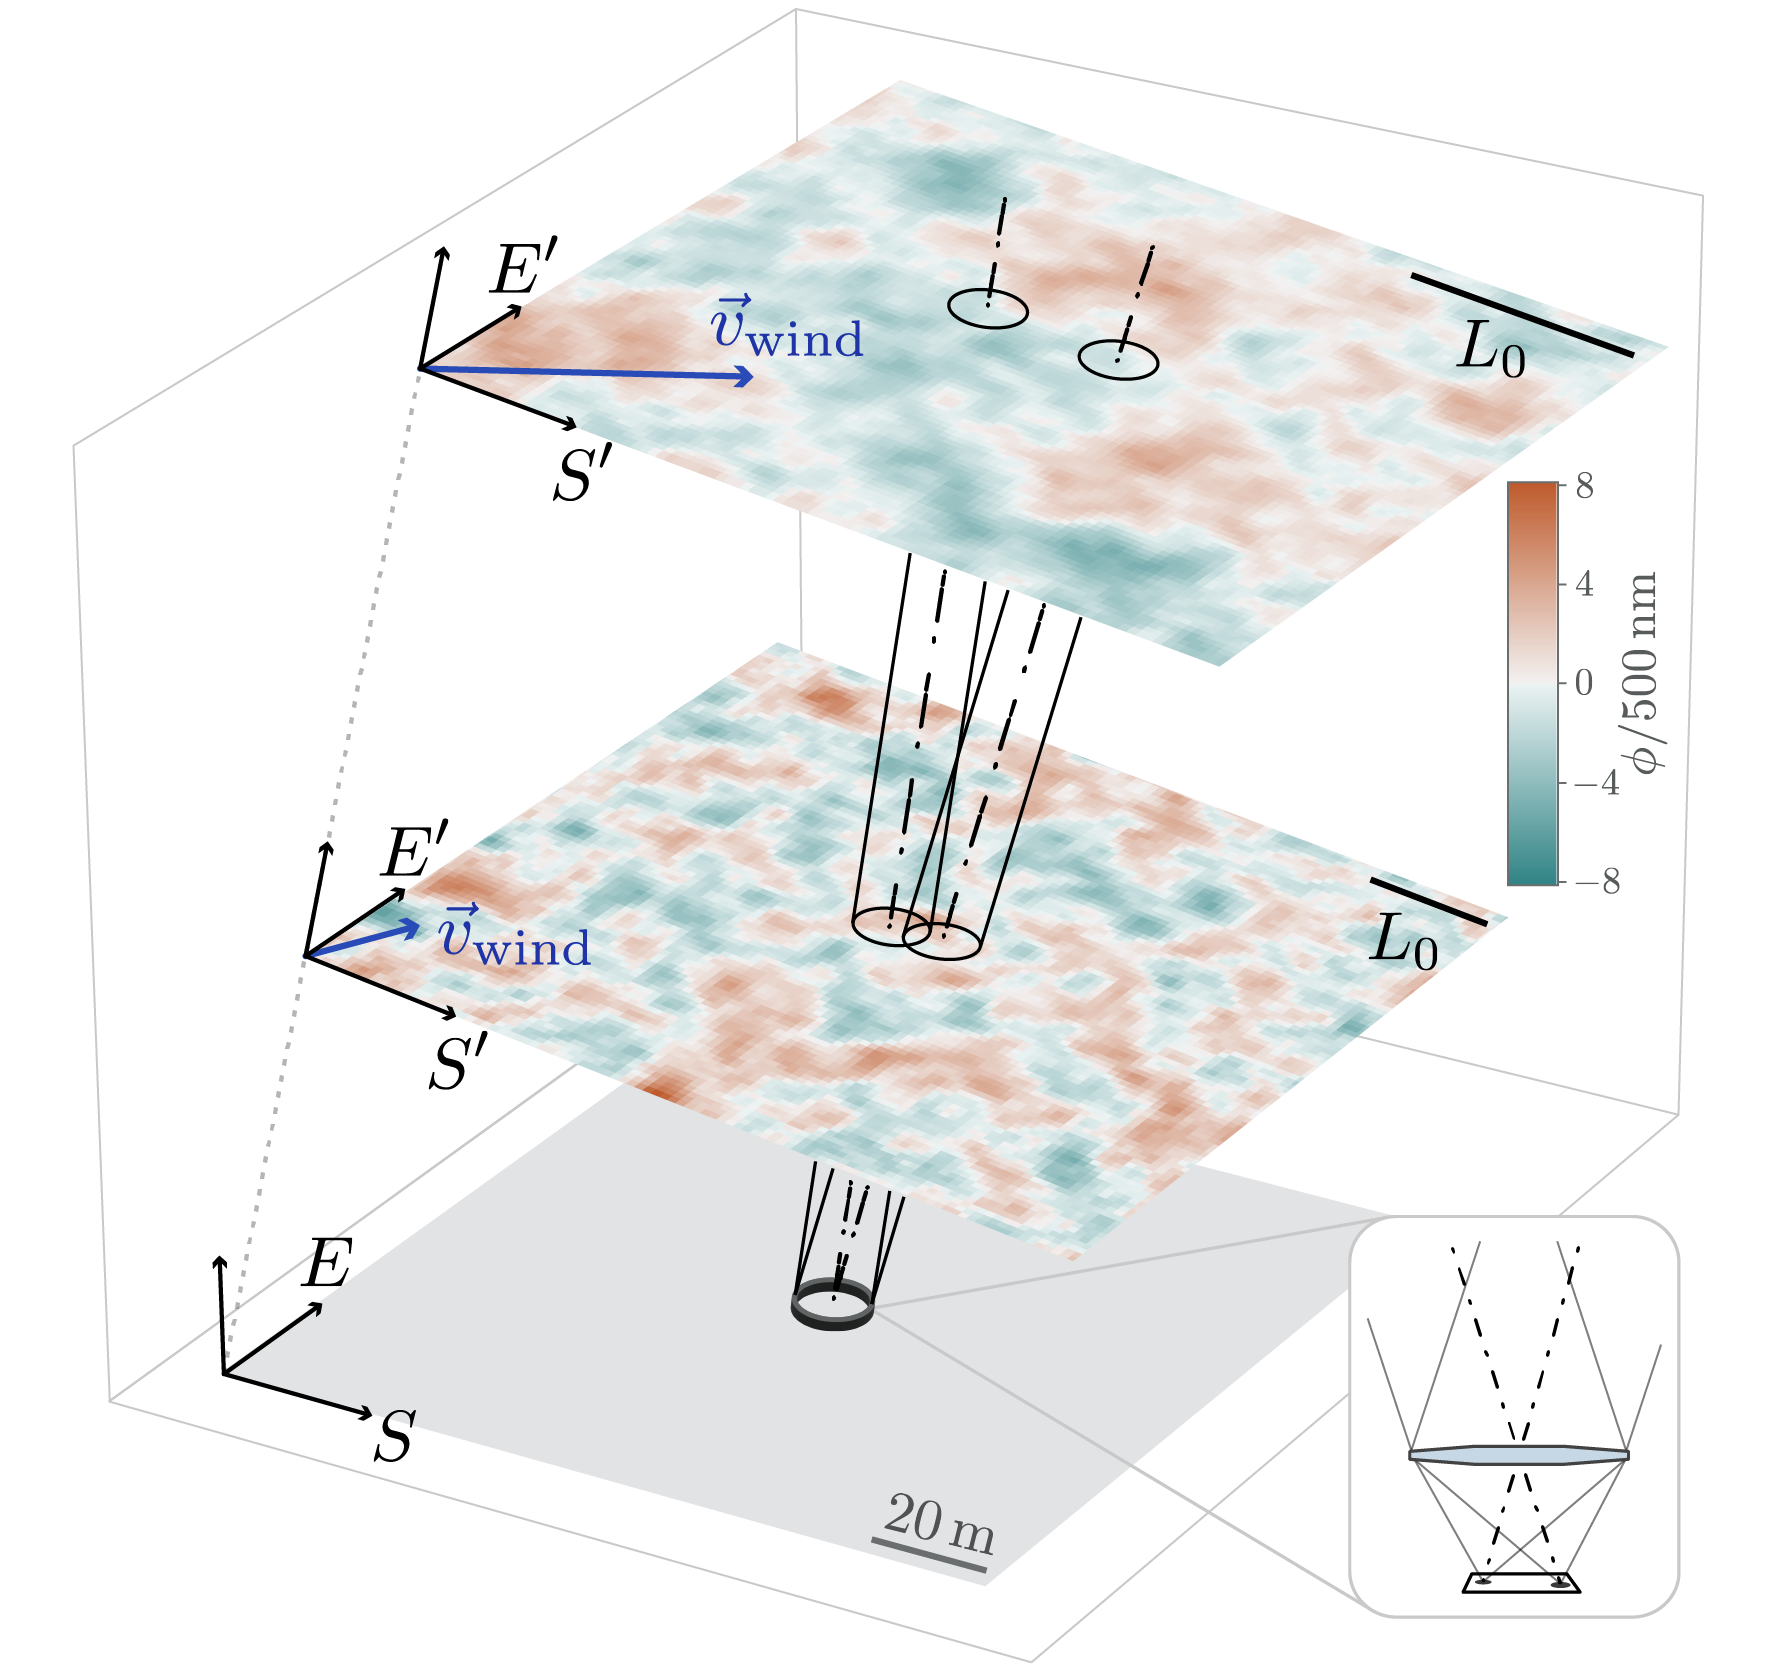
\includegraphics[width=0.45\textwidth]{f1_sim_schematic.png}
\caption{
    This schematic illustrates the simplified view of the atmosphere used for PSF simulations based on discrete phase screens. 
    Lines of sight (dot-dashed grey) for two stars (whose images are located at extrema of the field of view) pass through two phase screens of \vk refractive index variations, each with different values for the outer scale $L_0$. 
    The phase offset incurred by light passing through each point on each screen is indicated by the color scale in units of wavelength.
    The columns (teal) associated with each line of sight show the path of starlight that will reach the telescope aperture (black), along with the relevant phase screen area. 
    The wind vectors (orange arrows) show speed and direction of the wind in the plane of the screen.
    The primed coordinate systems are perpendicular to the telescope axis, and are related to the ground coordinate system via the altitude and azimuth of the pointing.
    \label{fig:schematic}
    }
\end{figure}

From this point, we will describe the details of  atmospheric PSF simulations in terms of the \galsim\footnote{\url{https://github.com/GalSim-developers/GalSim}} \citep{rowe_galsim_2015} implementation, but the principles hold for any workflow.
To set up the simulation of a single-exposure PSF (in the call to \texttt{galsim.Atmosphere}), one must define the environmental and turbulence parameters discussed above.
A building block of the simplified atmospheric model described above is the phase screen; one must define how many screens to include and, for each screen, set the following parameters: wind vector (speed and direction), altitude, outer scale, and turbulence integral contribution.

Turbulence strength is described in \galsim with the Fried parameter $r_0$, which determines the power spectrum amplitude for the total turbulence across all screens, and the relative weights $w_i$, which describe the contribution from each phase screen $i$ to the total turbulence integral $J$.
Turbulence integrals $J$ add linearly, so contributions to $r_0$ from each screen satisfy $r_0 = (\sum_{i} w_i r_0^{-5/3})^{-3/5}$\footnote{The $w_i$ parameter is denoted as $r_{0}\_$weights in \galsim, but they are really weights to the turbulence integral $J$.}.
By convention, the value of $r_0$ is specified for $\lambda=500\unit{nm}$ and zenith angle $\zeta=0$; the wavelength and zenith dependence of $r_0$ are used in \galsim to calculate the value of $r_0$ for other wavelengths and angles.

In this paper we adopt the meteorologic convention of defining wind direction; namely, wind direction describes the direction \textit{from} which the wind is blowing.
We define this angle in degrees East of North.
Unless otherwise specified, we will use ground coordinates for all parameters (the unprimed system in \figref{schematic}).

% Many of the quantities described above depend on the pointing of the telescope; the further off zenith, the more airmass present.

\section{\psfws overview} \label{sec:psfws}
A potential source of bias in weak lensing surveys is uncorrected, spatially correlated sources of noise. 
The atmosphere is correlated via the \vk power spectrum described in \eqnref{vk} and, as we have seen, these spatial correlations translate into angular correlations in the size and shape of the atmospheric PSF in the associated exposure.
Wind over the telescope plays an integral role in this process, as it moves correlated patches of turbulence through the atmospheric columns that  impact the images of different objects, leading to correlations on larger angular scales. 
Although wind varies with altitude, if wind directions are consistent across altitudes, turbulence at all altitudes will move coherently, thereby imprinting a stronger correlation in the PSF than when wind directions at different altitudes are uncorrelated. 
Another relevant factor for PSF correlations is the altitude-dependence of the optical turbulence profile (OTP), which describes the contribution of each layer to the total turbulence strength.
Interestingly, one of the drivers of atmospheric turbulence is wind itself -- specifically, wind shear -- so we expect that these two factors that influence spatial correlations in PSF parameters are not independent.

We separate the atmosphere into two regions based on the typical turbulence regime for those altitudes.
The ground layer (GL) is typically defined to be from ground level to $500-1000\unit{m}$ above the telescope; in this region, complex topography and heat sources generate non-Kolmogorov eddies.  The free atmosphere (FA) is the atmosphere above the ground layer; in this region, there are only a few sources of energy so turbulence is generally well-described by Kolmogorov statistics.
This separation into GL and FA plays an important role in many design choices for \psfws.

\subsection{guts of \psfws}

GCM provides wind profiles -- more about what GCMs are.
Problem: don't work so well for GL, which is a dominant contributor to the behavior of the PSF, including spatial correlations -- important to get right!
GCM limitations: unreliable parameters at ground, since interactions between the ground and the atmosphere will not be accurately captured, not to mention ground topography isn't high res, and grid is coarse so it's not actually telescope site. 

Osborn model provides empirical turbulence estimate (given temperature and pressure profiles, which can get from GCM) \FIXME{more about what it uses} -- validated on SCIDAR data \citep{osborn_optical_2018} at Cerro Paranal. 
Good, because mesoscale models are too slow (and more complex than we need).
Problem: doesn't work so well for GL because it assumes Komogorov behavior, it's very heuristic, and needs calibration of overall seeing.
% We will draw heavily from the heuristic forecasting model developed in \cite{osborn_atmospheric_2018} (hereafter \osborn, and note it's empirical!), itself adapting methods from mesoscale modeling develpoed by \cite{masciadri_optical_2017}. 
% Models turbulence strength at every altitude as a function of wind, pressure, and temperature gradients (they don't specify motivation; but one could expect $L(z)$ to depend on wind shear, since it will set how far two blobs of turbulence in adjacent altitudes can travel from each other horizontally, which is some measure of a maximum correlation length for turbulence), uses ECMWF as an input to this

% Despite the heuristic nature of this model, the turbulence model in \osborn seems to perform well for regions of weak turbulence, e.g. the free atmosphere, but significantly underpredicts ground layer turbulence (as expected, given the turbulence here is in general not weak) relative to the free atmosphere, given the median ground contribution of 60\% measured in T2005. 

% To achieve our goal of a predictive model for turbulence throughout the atmosphere which is correlated to environmental parameters in a realistic way, we will use \osborn

Can solve both these issues by also drawing on telemetry from telescope site. 
Weather tower provides ground wind information (time stamped, can match to GCM outputs) that can be used for GL screen -- but if not available, can still use package with ground layer information from GCM models.
Multiple GCM models run all over the globe, we have chosen to use the ERA5 reanalysis catalog of the European Center for Medium-range Weather Forecasts (ECMWF)\footnote{\url{https://www.ecmwf.int/en/forecasts/datasets/}} -- see \secref{gcm} for discussion on choice of weather forecasting dataset.

Suboptimal solution for turbulence: use MASS-DIMM measurements. 
Don't have a database of them (yet), but there are empirical PDFs in the literature, so use the FA value to calibrate Osborn OTP, and GL value as GL value. 
Plenty of evidence that FA and GL seeing are independent, so this is legit.
The sub-optimal part is the absence of temporal correlation between overall seeing and other weather parameters.

% Lots of empirical models based on microthermal balloon flights, SODAR, SLODAR, MASS/DIMM, SCIDAR, stereo-SCIDAR, etc (cite lots of papers here: Tokovinin 2003, Chun 2009, Els 2009, ...more in Zotero!)
% In particular, atmospheric PSF simulations in the literature commonly use the method of turbulence layers and weights set by Ellebroek (Alex M, Jee, DC2). 
% The limited data available did not allow for a description of variation in these layers or their turbulence integrals.
% With the addition of thousands of MASS+DIMM measurements to the dataset used in Ellebroek, Tokovinin 2005 improved on this model, providing three sets of weights, classified by quantiles of seeing quality, for a fixed number of altitude layers. 

% These studies and empirical models do not provide predictive capabilities for the optical turbulence, which is what we are after, but they provide useful information about the correlations between ground layer and free atmosphere turbulence, and between ground winds and seeing quality. 
% Three key takeaways from this literature are:
% \begin{enumerate}
%     \item the contributions to the turbulence integral from the ground layer and free atmosphere are independent from each other. T2005, Chun2009
%     \item the dependence of turbulence strength on wind speed: some evidence for this at ground, where turbulence triples in strength on average when wind speeds double from 7 to 15 m/s. 
%     Also some evidence for dependence of seeing on wind direction
%     \item Lastly, FA and GL seem to contribute roughly similar fractions to the overall seeing; this average behavior varies by location: GL is stronger (60\%) at CP and CT than MK (<50\%). And empirical levels for these distributions! T2005, Chun 2009, T2003
% \end{enumerate}

There is mixed evidence of correlations between wind speed and turbulence strength at the ground layer at various sites \FIXME{cite papers from lit rev}, so package can optionally take that as an input and match the turbulence draws to speeds to provide a statistically correlated distribution.


Turbulence layers are not fixed in altitude or number (cite Osborn SCIDAR paper) so we want these to vary in our outputs as well.
examples of how they are set in other papers, e.g. the ones cited in intro (Jee, Alex, etc)
Software can output parameters for any number of phase screens.
Can "place" phase screens in two different ways: middle of layer, or weighted by center of mass of turbulence within the layer.

Below, we summarize the steps conducted in \psfws, using Gemini-South at Cerro Pachón as an example observatory. 
This means we supply \psfws with telemetry from the weather tower at Gemini-S, ECMWF ERA5 data (the closest grid point to Cerra Pachón, at 30.2407$^{\circ}$S, 70.7366$^{\circ}$W, is at \CHECK{30.25$^{\circ}$S, 70.75$^{\circ}$W} -- this is \FIXME{X\unit{km}} away), and an empirical MASS+DIMM turbulence PDF from \FIXME{cite Tokovinin}. 

\CHECK{summarize the methods above in a numbered list, as below? use fig 2 as illustration}

First, load in data: match telemetry temporally to ECMWF values, and if correlation value is provided, generate $J_GL$ values and produce distribution correlated to speeds.
Then, given some point $p$ (the index of some data) package does the following to output a set of simulation-ready parameters:
\begin{enumerate}
\item get measured parameters for that date/time: $GL(p), FA(p)$
\item use \osborn model to calculate $C_n^2(h)$ from $FA(p)$
\item draw $J_{GL}, J_{FA}$ values from empirical PDF, use FA value to calibrate OTP
\item for the desired number of screens, calculate CoM (using $C_n^2(h)$ profile) height within each layer
\item interpolate parameters from the $GL(p), FA(p)$ measurements to the screen altitudes
\item integrate $C_n^2$ within altitude layers to find $J$ for each phase screens.
\end{enumerate}


\begin{figure}
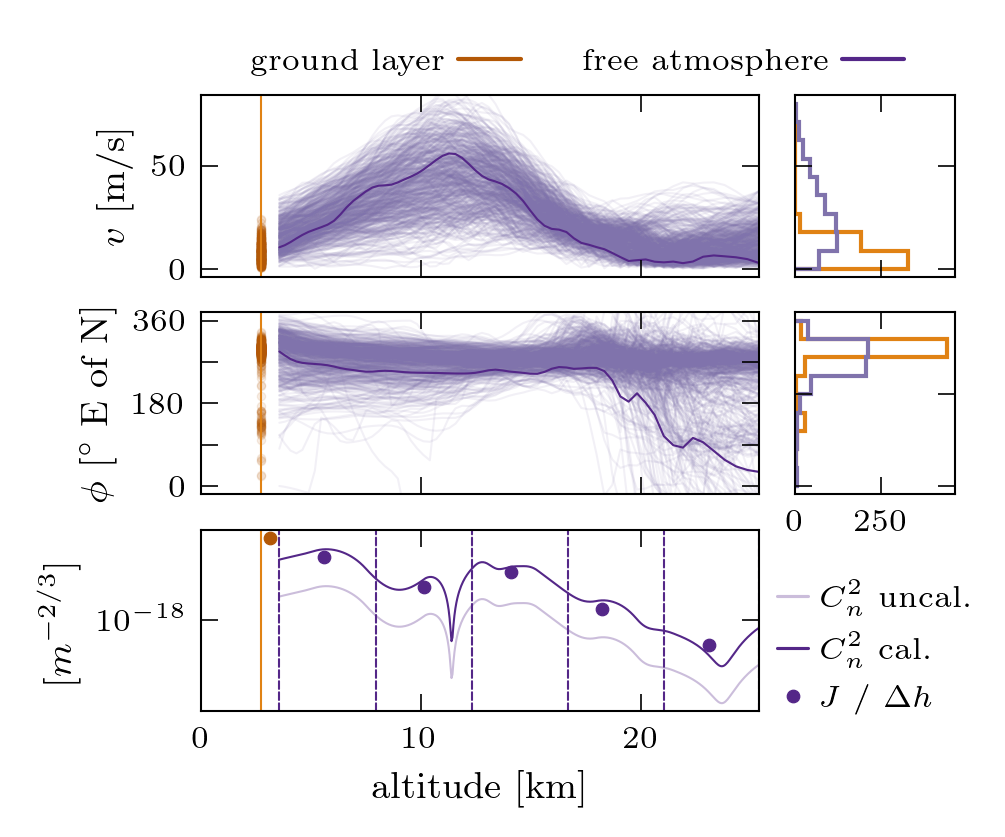
\includegraphics[width=0.47\textwidth]{f2_inputs.png}
\caption{Six months of wind data at and above Cerro Pach\'on (05/01/2019 to 11/01/2019), processed with \psfws as described in \secref{psfws}.
We plot wind speed (top) and meteorological direction (direction of wind \texit{origin}; middle) as a function of altitude, or as a frequency distribution on the right. 
Weather tower measurements of the ground layer (at an altitude of 50\unit{m}) are shown in orange; ECMWF ERA5 forecasts for the free atmosphere are shown in purple.
Temporal matching of the datasets is not depicted; however, each altitude profile in purple has a single co-temporal orange datapoint.
The heavy purple line in each panel corresponds to data from the same random timestamp.
In the bottom panel, the uncalibrated $C_n^2(h)$ profile for this example time is shown in light purple; scaled by $J_{FA}$, the calibrated profile is in dark purple. 
The dashed vertical lines depict the boundaries between the altitude bins used to calculate turbulence integrals $J$ for each FA phase screen.
Each $J$ is plotted scaled by the width of its corresponding altitude bin.
    \label{fig:inputs}
}

\end{figure}

\begin{figure}
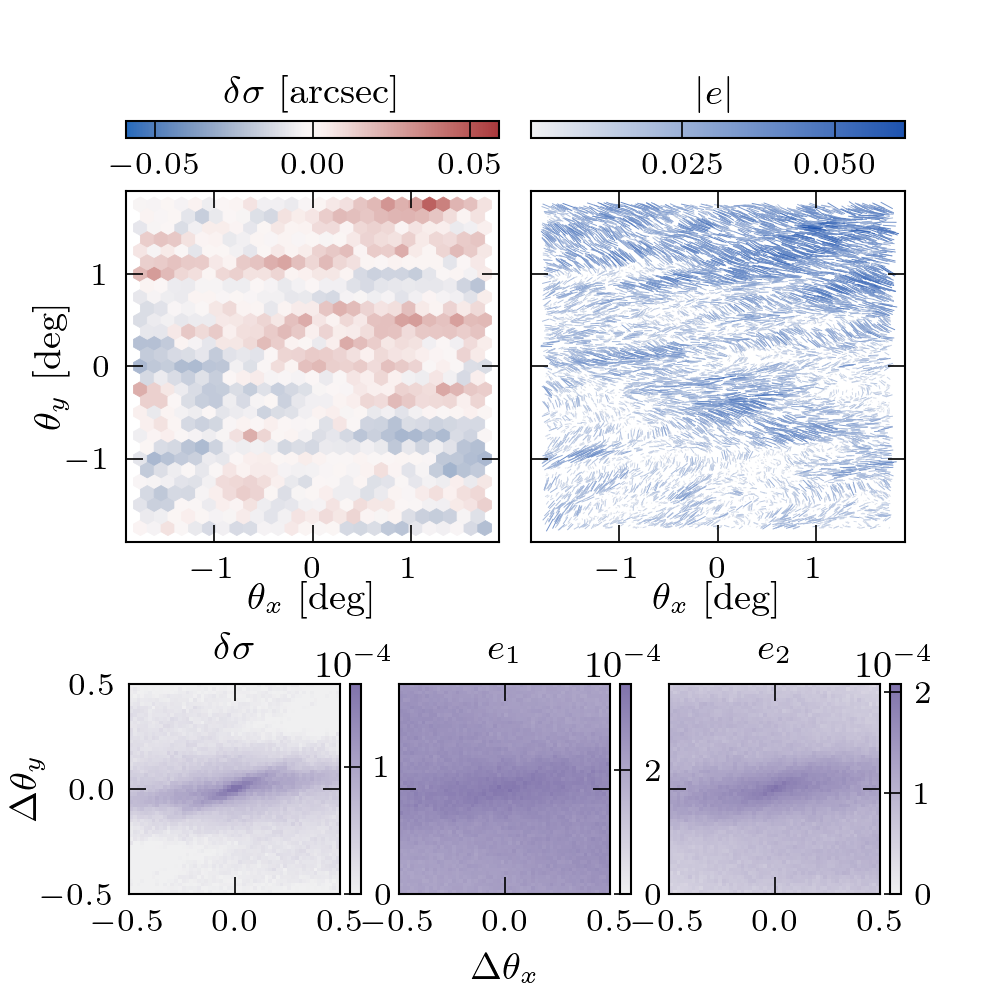
\includegraphics[width=0.47\textwidth]{f3_output.png}
\caption{
    \label{fig:output}
    }
\end{figure}

\section{Validation} \label{sec:valid}
The package described above draws from multiple sources of telemetry and vetted models. 
How do simulations run with \psfws vary from the previous generation of atmospheric PSF simulations? 
How do simulations run with \psfws compare to atmospheric PSFs osbserved at a survey telescope?
The section below addressed some of these questions, with simulations run as in \FIXME{cite DC2 paper} in \secref{imsimcompare} and with DES (optics-model subtracted) data in \secref{descompare}.

\subsection{Simulations at Cerro Pachon}\label{sec:imsimcompare}
How do simulations run with psfws inputs differ from those run with random inputs?

Comparison simulations are inputs from relevant literature: DC2 atmospheric simulations \FIXME{cite DC2 paper}: random distributions, variation on Ellerbroek.
Two variations on these: speeds as described in paper, and speeds matched to the limits of the data used for psfws as described above.

Simulations are run as follows:
pair (triplet?) of simulations use same seeing and atmospheric seed (ie turbulence generated is the same), same number of layers (set by imsim) and.... \CHECK{anything else?}
We don't expect anything from pairwise comparison of simulations, since we are interested in the comparison between the statistics of spatial correlations between the three sets of simulations.

To run comparison, compute moments of the anisotropic 2pcf maps of PSF parameters (size, shape). 
We use the following quantities to summarize each simulation result: the variance of the PSF parameter across the field of view, the "size" of the 2pcf ("correlation length"), and the "direction" of the 2pcf. 

\FIXME{plot: compare these three summary quantities for the 3 psf parameters for the three types of simulations}

\subsection{Data from Cerro Telolo} \label{sec:descompare}
How do simulations run with psfws at Cerro Telolo compare to DES optics-removed data?
coordinate swap between atm and \galsim


\section{Conclusion}
\begin{itemize}
    \item configuration details in github repo
    \item flexible model for simulation parameter generation -- code to download and format additional GCM data from either ECMWF or NOAA is included with the package; can do this for any location and duration (starting from...?). 
    \item (hopefully) reliably reproduces realistic correlations at CP
\end{itemize}

\begin{acknowledgments}
If Josh not author, thank him. Morgan and Mike J for code review, PF, Sowmya, Sid for discussions. J Osborn for sharing expertise. We acknowledge ECMWF for access to the weather forecast data through the MARS access system.

CSGF grant number, DARE funding

DESC blurb
\end{acknowledgments}

\vspace{5mm}
%% don't think I need to indicate any facilities here, even if I use a couple of public images/datasets from DES.
% \facilities{HST(STIS)} 

%% specify which programs were used during the creation of 
%% the manuscript. Authors should list each code and include either a
%% citation or url to the code inside ()s when available.

% \software{numpy, pandas, scipy, eecodes, ...}


\appendix
\section{Choice of GCM}\label{sec:gcm}
Multiple efforts across the world generating high-quality weather forecasts. 
A few different considerations affect the choice of dataset to use:
\begin{enumerate}
    \item Re-analysis vs forecast: many GCM models have "re-analysis" datasets available, which are past forecasts rerun with present-day state of the art numerical and data assimilation methods
    \item For our particular use case, useful to have high vertical spatial resolution available (the model levels sample 137 point in altitude) which enables us to capture important wind gradients in the atmosphere.
    \item horizontal spatial resolution: how far from observatory are you sampling
    \item temporal sampling: how frequently do you get model outputs?
\end{enumerate}

\FIXME{make a table summarizing ECMWF and NOAA datasets?}
The ERA5 data is available for each hour of the day and is sampled uniformly over the Earth's surface with 31km resolution. 

These two considerations led us to use the ERA5 reanalysis catalog of the European Center for Medium-range Weather Forecasts (ECMWF)\footnote{https://www.ecmwf.int/en/forecasts/datasets/}, although for dates after February 2022, the NOAA GFS is also available with the same vertical resolution.

ECMWF is a non-hydrostatic model, more details in \cite{osborn_atmospheric_2018} and...


\bibliography{references}{}
\bibliographystyle{aasjournal}

% use @misc for citing software or third party data repositories!
% \citet{2015ApJ...805...23C} provides a example of how the citation in the
% article references the external code at \doi{10.5281/zenodo.15991}

% \listofchanges

\end{document}